%--------------------
% Packages
% -------------------
\documentclass[11pt,english]{article}
\usepackage{amsfonts}
\usepackage[left=2.5cm,top=2cm,right=2.5cm,bottom=3cm,bindingoffset=0cm]{geometry}
\usepackage{amsmath, amsthm, amssymb}
\usepackage{tikz}
\usetikzlibrary{calc}
\usetikzlibrary{decorations.pathreplacing,calligraphy}
\usepackage{fancyhdr}
%\usepackage{currfile}
\usepackage{nicefrac}
\usepackage{cite}
\usepackage{graphicx}
\usepackage{caption}
\usepackage{longtable}
\usepackage{rotating}
\usepackage{lscape}
\usepackage{booktabs}
\usepackage{float}
\usepackage{placeins}
\usepackage{setspace}
\usepackage[font=itshape]{quoting}
\onehalfspacing
\usepackage{mathrsfs}
\usepackage{tcolorbox}
\usepackage{xcolor}
\usepackage{subcaption}
\usepackage{float}
\usepackage[multiple]{footmisc}
\usepackage[T1]{fontenc}
\usepackage[sc]{mathpazo}
\usepackage{listings}
\usepackage{longtable}
\definecolor{cmured}{RGB}{175,30,45}
\definecolor{macroblue}{RGB}{56,108,176}
\usepackage[format=plain,
            labelfont=bf,
            textfont=]{caption}
\usepackage[colorlinks=true,citecolor=macroblue,linkcolor=macroblue,urlcolor=macroblue]{hyperref}
\usepackage{varioref}
\usepackage{chngcntr}
\usepackage{datetime}

\definecolor{darkgreen}{RGB}{30,175,88}
\definecolor{darkblue}{RGB}{30,118,175}
\definecolor{maroon}{rgb}{0.66,0,0}
\definecolor{darkgreen}{rgb}{0,0.69,0}

%Counters
\newtheorem{theorem}{Theorem}[section] 
\newtheorem{proposition}{Proposition}
\newtheorem{lemma}{Lemma}
\newtheorem{corollary}{Corollary}
\newtheorem{assumption}{Assumption}
\newtheorem{axiom}{Axiom}
\newtheorem{case}{Case}
\newtheorem{claim}{Claim}
\newtheorem{condition}{Condition}
\newtheorem{definition}{Definition}
\newtheorem{example}{Example}
\newtheorem{notation}{Notation}
\newtheorem{remark}{Remark}


\hypersetup{ 	
pdfsubject = {},
pdftitle = {TidyTuesday Week 41},
pdfauthor = {Pranay Gundam},
linkcolor= macroblue
}


\title{\textbf{TidyTuesday Week 41}}
\author{Pranay Gundam}


%-----------------------
% Begin document
%-----------------------
\begin{document}

\maketitle

\tableofcontents

\section{Weekly Summary}


\section{Date: 2024-10-07}
\noindent \textbf{Series ID: HNOTASQ027S} 

\noindent This series is titled Households and nonprofit organizations; total assets, Level (DISCONTINUED) and has a frequency of Quarterly. The units are Millions of Dollars and the seasonal adjustment is Not Seasonally Adjusted.The observation start date is 1945-10-01 and the observation end date is 2017-10-01.The popularity of this series is 1. \\ 

\noindent \textbf{Series ID: QFR215323USNO} 

\noindent This series is titled Quarterly Financial Report: U.S. Corporations: Printing and Related Support Activities: All Other Current Assets and has a frequency of Quarterly. The units are Millions of Dollars and the seasonal adjustment is Not Seasonally Adjusted.The observation start date is 2000-10-01 and the observation end date is 2024-04-01.The popularity of this series is 0. \\ 

\subsection{Regression Tables and Plots}
\begin{center}
\begin{tabular}{lclc}
\toprule
\textbf{Dep. Variable:}           & value\_fred\_QFR215323USNO & \textbf{  R-squared:         } &     0.163   \\
\textbf{Model:}                   &            OLS             & \textbf{  Adj. R-squared:    } &     0.150   \\
\textbf{Method:}                  &       Least Squares        & \textbf{  F-statistic:       } &     13.03   \\
\textbf{Date:}                    &      Mon, 07 Oct 2024      & \textbf{  Prob (F-statistic):} &  0.000586   \\
\textbf{Time:}                    &          11:43:35          & \textbf{  Log-Likelihood:    } &   -467.21   \\
\textbf{No. Observations:}        &               69           & \textbf{  AIC:               } &     938.4   \\
\textbf{Df Residuals:}            &               67           & \textbf{  BIC:               } &     942.9   \\
\textbf{Df Model:}                &                1           & \textbf{                     } &             \\
\textbf{Covariance Type:}         &         nonrobust          & \textbf{                     } &             \\
\bottomrule
\end{tabular}
\begin{tabular}{lcccccc}
                                  & \textbf{coef} & \textbf{std err} & \textbf{t} & \textbf{P$> |$t$|$} & \textbf{[0.025} & \textbf{0.975]}  \\
\midrule
\textbf{const}                    &    1227.7900  &      118.614     &    10.351  &         0.000        &      991.035    &     1464.545     \\
\textbf{value\_fred\_HNOTASQ027S} &    5.376e-06  &     1.49e-06     &     3.610  &         0.001        &      2.4e-06    &     8.35e-06     \\
\bottomrule
\end{tabular}
\begin{tabular}{lclc}
\textbf{Omnibus:}       & 11.288 & \textbf{  Durbin-Watson:     } &    0.852  \\
\textbf{Prob(Omnibus):} &  0.004 & \textbf{  Jarque-Bera (JB):  } &    4.001  \\
\textbf{Skew:}          &  0.269 & \textbf{  Prob(JB):          } &    0.135  \\
\textbf{Kurtosis:}      &  1.950 & \textbf{  Cond. No.          } & 3.66e+08  \\
\bottomrule
\end{tabular}
%\caption{OLS Regression Results}
\end{center}

Notes: \newline
 [1] Standard Errors assume that the covariance matrix of the errors is correctly specified. \newline
 [2] The condition number is large, 3.66e+08. This might indicate that there are \newline
 strong multicollinearity or other numerical problems.

\begin{figure}
\centering
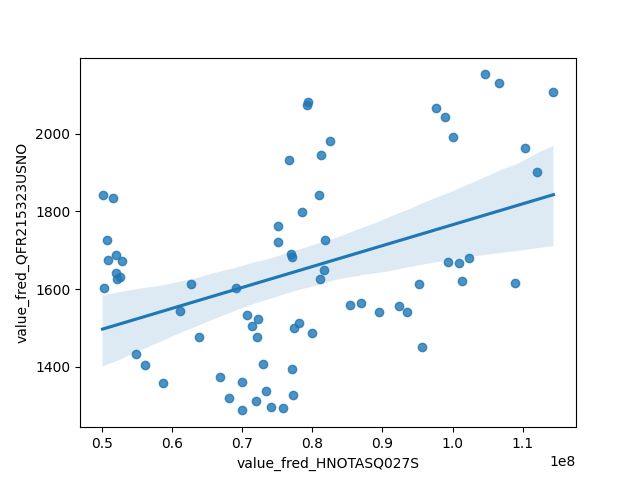
\includegraphics[scale = 0.9]{plots/plot_2024-10-07.png}
\caption{Regression Plot for 2024-10-07}
\end{figure}
\newpage

\section{Date: 2024-10-08}
\noindent \textbf{Series ID: IPUGN42421U110000000} 

\noindent This series is titled Labor Compensation for Wholesale Trade: Drugs and Druggists' Sundries Merchant Wholesalers (NAICS 42421) in the United States and has a frequency of Annual. The units are Index 2017=100 and the seasonal adjustment is Not Seasonally Adjusted.The observation start date is 1987-01-01 and the observation end date is 2023-01-01.The popularity of this series is 0. \\ 

\noindent \textbf{Series ID: NZLRECM} 

\noindent This series is titled OECD based Recession Indicators for New Zealand from the Peak through the Trough and has a frequency of Monthly. The units are +1 or 0 and the seasonal adjustment is Not Seasonally Adjusted.The observation start date is 1960-02-01 and the observation end date is 2017-10-01.The popularity of this series is 2. \\ 

\subsection{Regression Tables and Plots}
\begin{center}
\begin{tabular}{lclc}
\toprule
\textbf{Dep. Variable:}                    & value\_fred\_NZLRECM & \textbf{  R-squared:         } &     0.024   \\
\textbf{Model:}                            &         OLS          & \textbf{  Adj. R-squared:    } &    -0.010   \\
\textbf{Method:}                           &    Least Squares     & \textbf{  F-statistic:       } &    0.7055   \\
\textbf{Date:}                             &   Tue, 08 Oct 2024   & \textbf{  Prob (F-statistic):} &    0.408    \\
\textbf{Time:}                             &       10:11:56       & \textbf{  Log-Likelihood:    } &   -21.981   \\
\textbf{No. Observations:}                 &            31        & \textbf{  AIC:               } &     47.96   \\
\textbf{Df Residuals:}                     &            29        & \textbf{  BIC:               } &     50.83   \\
\textbf{Df Model:}                         &             1        & \textbf{                     } &             \\
\textbf{Covariance Type:}                  &      nonrobust       & \textbf{                     } &             \\
\bottomrule
\end{tabular}
\begin{tabular}{lcccccc}
                                           & \textbf{coef} & \textbf{std err} & \textbf{t} & \textbf{P$> |$t$|$} & \textbf{[0.025} & \textbf{0.975]}  \\
\midrule
\textbf{const}                             &       0.5963  &        0.195     &     3.058  &         0.005        &        0.198    &        0.995     \\
\textbf{value\_fred\_IPUGN42421U110000000} &      -0.0026  &        0.003     &    -0.840  &         0.408        &       -0.009    &        0.004     \\
\bottomrule
\end{tabular}
\begin{tabular}{lclc}
\textbf{Omnibus:}       & 98.779 & \textbf{  Durbin-Watson:     } &    1.730  \\
\textbf{Prob(Omnibus):} &  0.000 & \textbf{  Jarque-Bera (JB):  } &    4.694  \\
\textbf{Skew:}          &  0.183 & \textbf{  Prob(JB):          } &   0.0956  \\
\textbf{Kurtosis:}      &  1.129 & \textbf{  Cond. No.          } &     136.  \\
\bottomrule
\end{tabular}
%\caption{OLS Regression Results}
\end{center}

Notes: \newline
 [1] Standard Errors assume that the covariance matrix of the errors is correctly specified.

\begin{figure}
\centering
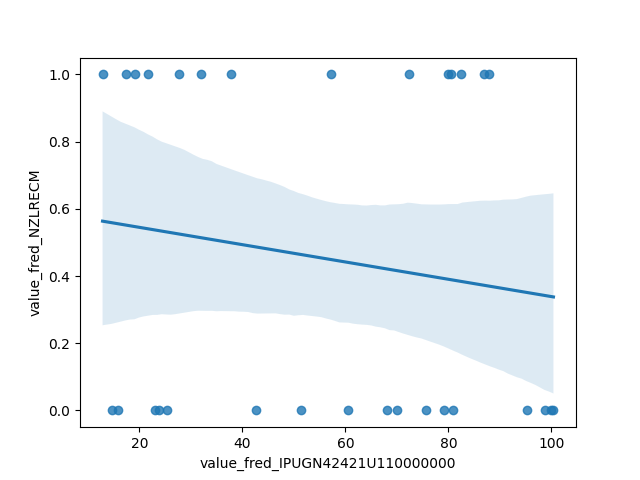
\includegraphics[scale = 0.9]{plots/plot_2024-10-08.png}
\caption{Regression Plot for 2024-10-08}
\end{figure}
\newpage

\section{Date: 2024-10-09}
\noindent \textbf{Series ID: ESTSFXFBNQ} 

\noindent This series is titled Percent of Value of Loans Secured by Collateral by Time that Pricing Terms Were Set and by Commitment, During Survey Week, Formal Commitment, U.S. Branches and Agencies of Foreign Banks (DISCONTINUED) and has a frequency of Quarterly, 2nd Month's 1st Full Week. The units are Percent and the seasonal adjustment is Not Seasonally Adjusted.The observation start date is 2003-07-01 and the observation end date is 2017-04-01.The popularity of this series is 0. \\ 

\noindent \textbf{Series ID: CIS2027200000000I} 

\noindent This series is titled Employment Cost Index: Wages and salaries for Private industry workers in Accommodations and food service and has a frequency of Quarterly. The units are Index Dec 2005=100 and the seasonal adjustment is Seasonally Adjusted.The observation start date is 2003-01-01 and the observation end date is 2024-04-01.The popularity of this series is 8. \\ 

\subsection{Regression Tables and Plots}
\begin{center}
\begin{tabular}{lclc}
\toprule
\textbf{Dep. Variable:}          & value\_fred\_CIS2027200000000I & \textbf{  R-squared:         } &     0.008   \\
\textbf{Model:}                  &              OLS               & \textbf{  Adj. R-squared:    } &    -0.010   \\
\textbf{Method:}                 &         Least Squares          & \textbf{  F-statistic:       } &    0.4473   \\
\textbf{Date:}                   &        Wed, 09 Oct 2024        & \textbf{  Prob (F-statistic):} &    0.506    \\
\textbf{Time:}                   &            20:31:41            & \textbf{  Log-Likelihood:    } &   -206.44   \\
\textbf{No. Observations:}       &                 56             & \textbf{  AIC:               } &     416.9   \\
\textbf{Df Residuals:}           &                 54             & \textbf{  BIC:               } &     420.9   \\
\textbf{Df Model:}               &                  1             & \textbf{                     } &             \\
\textbf{Covariance Type:}        &           nonrobust            & \textbf{                     } &             \\
\bottomrule
\end{tabular}
\begin{tabular}{lcccccc}
                                 & \textbf{coef} & \textbf{std err} & \textbf{t} & \textbf{P$> |$t$|$} & \textbf{[0.025} & \textbf{0.975]}  \\
\midrule
\textbf{const}                   &     114.2979  &        2.585     &    44.213  &         0.000        &      109.115    &      119.481     \\
\textbf{value\_fred\_ESTSFXFBNQ} &      -0.0452  &        0.068     &    -0.669  &         0.506        &       -0.181    &        0.090     \\
\bottomrule
\end{tabular}
\begin{tabular}{lclc}
\textbf{Omnibus:}       &  1.970 & \textbf{  Durbin-Watson:     } &    0.018  \\
\textbf{Prob(Omnibus):} &  0.373 & \textbf{  Jarque-Bera (JB):  } &    1.410  \\
\textbf{Skew:}          & -0.157 & \textbf{  Prob(JB):          } &    0.494  \\
\textbf{Kurtosis:}      &  2.289 & \textbf{  Cond. No.          } &     75.2  \\
\bottomrule
\end{tabular}
%\caption{OLS Regression Results}
\end{center}

Notes: \newline
 [1] Standard Errors assume that the covariance matrix of the errors is correctly specified.

\begin{figure}
\centering
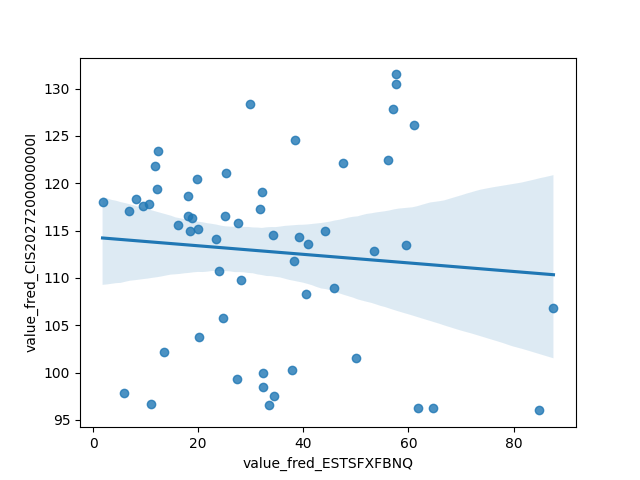
\includegraphics[scale = 0.9]{plots/plot_2024-10-09.png}
\caption{Regression Plot for 2024-10-09}
\end{figure}
\newpage

\section{Date: 2024-10-10}
\noindent \textbf{Series ID: TLRESCON} 

\noindent This series is titled Total Construction Spending: Residential in the United States and has a frequency of Monthly. The units are Millions of Dollars and the seasonal adjustment is Not Seasonally Adjusted.The observation start date is 2002-01-01 and the observation end date is 2024-08-01.The popularity of this series is 15. \\ 

\noindent \textbf{Series ID: NENGPETCOALMANRGSP} 

\noindent This series is titled Real Gross Domestic Product: Petroleum and Coal Products Manufacturing (324) in the New England BEA Region and has a frequency of Annual. The units are Millions of Chained 2017 Dollars and the seasonal adjustment is Not Seasonally Adjusted.The observation start date is 1997-01-01 and the observation end date is 2023-01-01.The popularity of this series is 0. \\ 

\subsection{Regression Tables and Plots}
\begin{center}
\begin{tabular}{lclc}
\toprule
\textbf{Dep. Variable:}        & value\_fred\_NENGPETCOALMANRGSP & \textbf{  R-squared:         } &     0.001   \\
\textbf{Model:}                &               OLS               & \textbf{  Adj. R-squared:    } &    -0.049   \\
\textbf{Method:}               &          Least Squares          & \textbf{  F-statistic:       } &   0.01225   \\
\textbf{Date:}                 &         Thu, 10 Oct 2024        & \textbf{  Prob (F-statistic):} &    0.913    \\
\textbf{Time:}                 &             09:54:26            & \textbf{  Log-Likelihood:    } &   -152.56   \\
\textbf{No. Observations:}     &                  22             & \textbf{  AIC:               } &     309.1   \\
\textbf{Df Residuals:}         &                  20             & \textbf{  BIC:               } &     311.3   \\
\textbf{Df Model:}             &                   1             & \textbf{                     } &             \\
\textbf{Covariance Type:}      &            nonrobust            & \textbf{                     } &             \\
\bottomrule
\end{tabular}
\begin{tabular}{lcccccc}
                               & \textbf{coef} & \textbf{std err} & \textbf{t} & \textbf{P$> |$t$|$} & \textbf{[0.025} & \textbf{0.975]}  \\
\midrule
\textbf{const}                 &     741.9514  &      154.524     &     4.802  &         0.000        &      419.621    &     1064.282     \\
\textbf{value\_fred\_TLRESCON} &       0.0005  &        0.004     &     0.111  &         0.913        &       -0.008    &        0.009     \\
\bottomrule
\end{tabular}
\begin{tabular}{lclc}
\textbf{Omnibus:}       &  6.858 & \textbf{  Durbin-Watson:     } &    0.615  \\
\textbf{Prob(Omnibus):} &  0.032 & \textbf{  Jarque-Bera (JB):  } &    4.737  \\
\textbf{Skew:}          &  1.082 & \textbf{  Prob(JB):          } &   0.0936  \\
\textbf{Kurtosis:}      &  3.693 & \textbf{  Cond. No.          } & 1.01e+05  \\
\bottomrule
\end{tabular}
%\caption{OLS Regression Results}
\end{center}

Notes: \newline
 [1] Standard Errors assume that the covariance matrix of the errors is correctly specified. \newline
 [2] The condition number is large, 1.01e+05. This might indicate that there are \newline
 strong multicollinearity or other numerical problems.

\begin{figure}
\centering
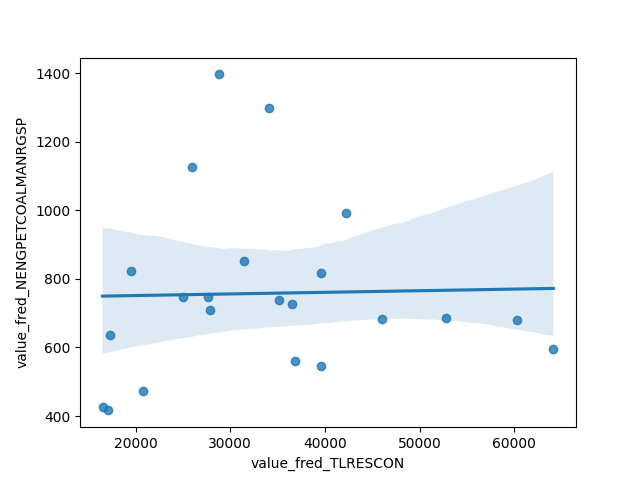
\includegraphics[scale = 0.9]{plots/plot_2024-10-10.png}
\caption{Regression Plot for 2024-10-10}
\end{figure}
\newpage

\section{Date: 2024-10-11}
\noindent \textbf{Series ID: BNEMFT01KRQ460S} 

\noindent This series is titled Business Tendency Surveys for Non-Manufacturing: Employment: Future Tendency: National Indicator for the Republic of Korea (DISCONTINUED) and has a frequency of Quarterly. The units are Net Percent and the seasonal adjustment is Seasonally Adjusted.The observation start date is 1993-01-01 and the observation end date is 2003-01-01.The popularity of this series is 1. \\ 

\noindent \textbf{Series ID: THREEFFTP6} 

\noindent This series is titled Instantaneous Forward Term Premium 6 Years Hence and has a frequency of Daily. The units are Percent and the seasonal adjustment is Not Seasonally Adjusted.The observation start date is 1990-01-02 and the observation end date is 2024-10-04.The popularity of this series is 2. \\ 

\subsection{Regression Tables and Plots}
\begin{center}
\begin{tabular}{lclc}
\toprule
\textbf{Dep. Variable:}               & value\_fred\_THREEFFTP6 & \textbf{  R-squared:         } &     0.488   \\
\textbf{Model:}                       &           OLS           & \textbf{  Adj. R-squared:    } &     0.459   \\
\textbf{Method:}                      &      Least Squares      & \textbf{  F-statistic:       } &     17.14   \\
\textbf{Date:}                        &     Fri, 11 Oct 2024    & \textbf{  Prob (F-statistic):} &  0.000614   \\
\textbf{Time:}                        &         14:58:58        & \textbf{  Log-Likelihood:    } &   -3.4076   \\
\textbf{No. Observations:}            &              20         & \textbf{  AIC:               } &     10.82   \\
\textbf{Df Residuals:}                &              18         & \textbf{  BIC:               } &     12.81   \\
\textbf{Df Model:}                    &               1         & \textbf{                     } &             \\
\textbf{Covariance Type:}             &        nonrobust        & \textbf{                     } &             \\
\bottomrule
\end{tabular}
\begin{tabular}{lcccccc}
                                      & \textbf{coef} & \textbf{std err} & \textbf{t} & \textbf{P$> |$t$|$} & \textbf{[0.025} & \textbf{0.975]}  \\
\midrule
\textbf{const}                        &       1.3795  &        0.088     &    15.636  &         0.000        &        1.194    &        1.565     \\
\textbf{value\_fred\_BNEMFT01KRQ460S} &      -0.0328  &        0.008     &    -4.140  &         0.001        &       -0.049    &       -0.016     \\
\bottomrule
\end{tabular}
\begin{tabular}{lclc}
\textbf{Omnibus:}       &  2.364 & \textbf{  Durbin-Watson:     } &    1.557  \\
\textbf{Prob(Omnibus):} &  0.307 & \textbf{  Jarque-Bera (JB):  } &    0.806  \\
\textbf{Skew:}          & -0.193 & \textbf{  Prob(JB):          } &    0.668  \\
\textbf{Kurtosis:}      &  3.905 & \textbf{  Cond. No.          } &     14.6  \\
\bottomrule
\end{tabular}
%\caption{OLS Regression Results}
\end{center}

Notes: \newline
 [1] Standard Errors assume that the covariance matrix of the errors is correctly specified.

\begin{figure}
\centering
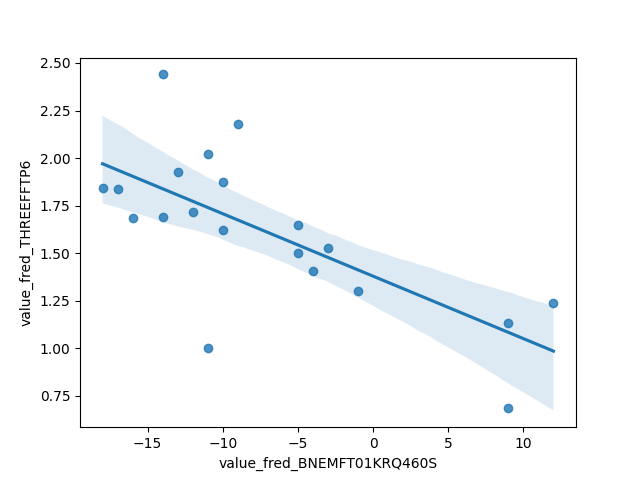
\includegraphics[scale = 0.9]{plots/plot_2024-10-11.png}
\caption{Regression Plot for 2024-10-11}
\end{figure}
\newpage

\section{Date: 2024-10-12}
\noindent \textbf{Series ID: EEMMXSSNQ} 

\noindent This series is titled Weighted-Average Effective Loan Rate for 31 to 365 Days, Moderate Risk, Small Domestic Banks (DISCONTINUED) and has a frequency of Quarterly, 2nd Month's 1st Full Week. The units are Percent and the seasonal adjustment is Not Seasonally Adjusted.The observation start date is 1997-04-01 and the observation end date is 2017-04-01.The popularity of this series is 1. \\ 

\noindent \textbf{Series ID: A842RL1Q225SBEA} 

\noindent This series is titled Real Government Gross Investment: State and Local: Gross Investment: Structures and has a frequency of Quarterly. The units are Percent Change from Preceding Period and the seasonal adjustment is Seasonally Adjusted Annual Rate.The observation start date is 1947-04-01 and the observation end date is 2024-04-01.The popularity of this series is 1. \\ 

\subsection{Regression Tables and Plots}
\begin{center}
\begin{tabular}{lclc}
\toprule
\textbf{Dep. Variable:}         & value\_fred\_A842RL1Q225SBEA & \textbf{  R-squared:         } &     0.029   \\
\textbf{Model:}                 &             OLS              & \textbf{  Adj. R-squared:    } &     0.016   \\
\textbf{Method:}                &        Least Squares         & \textbf{  F-statistic:       } &     2.321   \\
\textbf{Date:}                  &       Sat, 12 Oct 2024       & \textbf{  Prob (F-statistic):} &    0.132    \\
\textbf{Time:}                  &           23:51:33           & \textbf{  Log-Likelihood:    } &   -303.96   \\
\textbf{No. Observations:}      &                81            & \textbf{  AIC:               } &     611.9   \\
\textbf{Df Residuals:}          &                79            & \textbf{  BIC:               } &     616.7   \\
\textbf{Df Model:}              &                 1            & \textbf{                     } &             \\
\textbf{Covariance Type:}       &          nonrobust           & \textbf{                     } &             \\
\bottomrule
\end{tabular}
\begin{tabular}{lcccccc}
                                & \textbf{coef} & \textbf{std err} & \textbf{t} & \textbf{P$> |$t$|$} & \textbf{[0.025} & \textbf{0.975]}  \\
\midrule
\textbf{const}                  &      -6.5483  &        4.891     &    -1.339  &         0.184        &      -16.283    &        3.187     \\
\textbf{value\_fred\_EEMMXSSNQ} &       1.1106  &        0.729     &     1.524  &         0.132        &       -0.340    &        2.562     \\
\bottomrule
\end{tabular}
\begin{tabular}{lclc}
\textbf{Omnibus:}       & 14.862 & \textbf{  Durbin-Watson:     } &    2.362  \\
\textbf{Prob(Omnibus):} &  0.001 & \textbf{  Jarque-Bera (JB):  } &   23.904  \\
\textbf{Skew:}          &  0.713 & \textbf{  Prob(JB):          } & 6.44e-06  \\
\textbf{Kurtosis:}      &  5.247 & \textbf{  Cond. No.          } &     28.9  \\
\bottomrule
\end{tabular}
%\caption{OLS Regression Results}
\end{center}

Notes: \newline
 [1] Standard Errors assume that the covariance matrix of the errors is correctly specified.

\begin{figure}
\centering
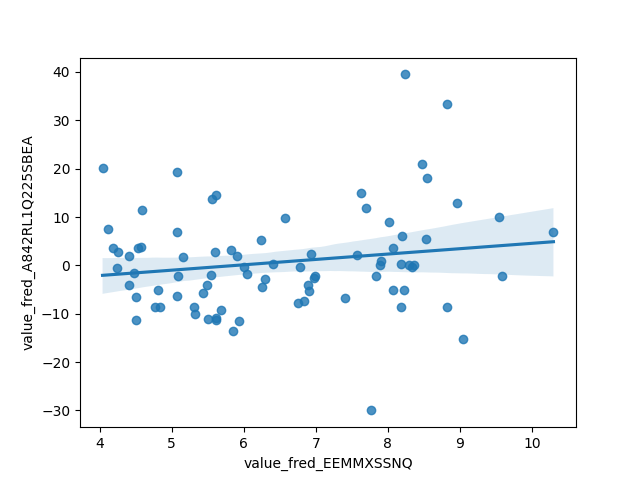
\includegraphics[scale = 0.9]{plots/plot_2024-10-12.png}
\caption{Regression Plot for 2024-10-12}
\end{figure}
\newpage

\section{Date: 2024-10-13}
\noindent \textbf{Series ID: BOPMPA} 

\noindent This series is titled Other Private Income Payments on Foreign Assets in U.S. (DISCONTINUED) and has a frequency of Annual. The units are Billions of Dollars and the seasonal adjustment is Not Seasonally Adjusted.The observation start date is 1960-01-01 and the observation end date is 2013-01-01.The popularity of this series is 0. \\ 

\noindent \textbf{Series ID: BOPGPN} 

\noindent This series is titled U.S. Government Pensions and Other Transfers (DISCONTINUED) and has a frequency of Quarterly. The units are Billions of Dollars and the seasonal adjustment is Not Seasonally Adjusted.The observation start date is 1960-01-01 and the observation end date is 2014-01-01.The popularity of this series is 1. \\ 

\subsection{Regression Tables and Plots}
\begin{center}
\begin{tabular}{lclc}
\toprule
\textbf{Dep. Variable:}      & value\_fred\_BOPGPN & \textbf{  R-squared:         } &     0.616   \\
\textbf{Model:}              &         OLS         & \textbf{  Adj. R-squared:    } &     0.609   \\
\textbf{Method:}             &    Least Squares    & \textbf{  F-statistic:       } &     83.40   \\
\textbf{Date:}               &   Sun, 13 Oct 2024  & \textbf{  Prob (F-statistic):} &  2.17e-12   \\
\textbf{Time:}               &       10:12:43      & \textbf{  Log-Likelihood:    } &   -14.582   \\
\textbf{No. Observations:}   &            54       & \textbf{  AIC:               } &     33.16   \\
\textbf{Df Residuals:}       &            52       & \textbf{  BIC:               } &     37.14   \\
\textbf{Df Model:}           &             1       & \textbf{                     } &             \\
\textbf{Covariance Type:}    &      nonrobust      & \textbf{                     } &             \\
\bottomrule
\end{tabular}
\begin{tabular}{lcccccc}
                             & \textbf{coef} & \textbf{std err} & \textbf{t} & \textbf{P$> |$t$|$} & \textbf{[0.025} & \textbf{0.975]}  \\
\midrule
\textbf{const}               &      -0.2816  &        0.058     &    -4.854  &         0.000        &       -0.398    &       -0.165     \\
\textbf{value\_fred\_BOPMPA} &       0.0040  &        0.000     &     9.132  &         0.000        &        0.003    &        0.005     \\
\bottomrule
\end{tabular}
\begin{tabular}{lclc}
\textbf{Omnibus:}       & 18.507 & \textbf{  Durbin-Watson:     } &    1.255  \\
\textbf{Prob(Omnibus):} &  0.000 & \textbf{  Jarque-Bera (JB):  } &   56.564  \\
\textbf{Skew:}          &  0.747 & \textbf{  Prob(JB):          } & 5.21e-13  \\
\textbf{Kurtosis:}      &  7.786 & \textbf{  Cond. No.          } &     176.  \\
\bottomrule
\end{tabular}
%\caption{OLS Regression Results}
\end{center}

Notes: \newline
 [1] Standard Errors assume that the covariance matrix of the errors is correctly specified.

\begin{figure}
\centering
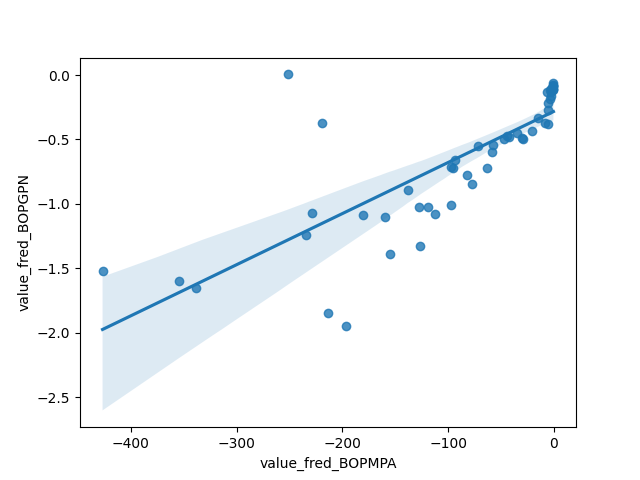
\includegraphics[scale = 0.9]{plots/plot_2024-10-13.png}
\caption{Regression Plot for 2024-10-13}
\end{figure}
\newpage


\end{document}
